% rubber: module pdftex

\documentclass[a4paper,11pt]{article}
\usepackage[top = 1.5 in, bottom = 1 in, left = 1 in, right = 1 in]{geometry}
\usepackage[utf8]{inputenc}
\usepackage[T1]{fontenc}
\usepackage{csquotes}
\usepackage[british]{babel}
\usepackage{lmodern}
\usepackage{url}
\usepackage{color}
\usepackage{graphicx}
\usepackage{setspace}
\usepackage{pdfpages}
\usepackage{amsmath}

\begin{document}
\title{Compiler project: MiniJava}
\author{Laura Leppänen \\ Compilers, Spring 2012}
\date{\today}
\maketitle
\thispagestyle{empty}

\tableofcontents
\onehalfspacing

\newpage
\setcounter{page}{1}

\section{The Mini-Java language}

\subsection{Token patterns}

Defined using regular expressions with Java style character classes. These token groups correspond to token classes used in the implementation.

\begin{description}
\item[Identifiers] $\backslash\text{p\{IsAlphabetic\}} [ \backslash\text{p\{IsAlphabetic\}}\backslash\text{p\{IsDigit\}\_ } ]^{*}$ \\ \emph{Except simple types and keywords.}
\item[Integer literals] $\backslash\text{p\{IsDigit\}}^{+}$
\item[Simple type] int | boolean | void
\item[Keyword] class | public | static | main | extends | assert | if | else | \\ while | System | out | println | return | new | length | this | true | false
\item[Operator] \&\& | || | < | > | == | + | - | *  | / | \% | = | !
\item[Punctuation] \{ | \} | [ | ] | ( | ) | $\backslash$. | ; | ,
\end{description}

\subsection{Modified grammar for recursive descent parsing (non-LL(1))}

In the grammar below, I have solved operator precedences using the ``classical'' method of making a separate production rule for each level of operator precedence. This is very easy to implement in the case of Mini-Java especially since all the defined binary operators are left-associative and there is only one unary operator. In a more complex case something like the Shunting Yard algorithm would probably work better.\footnote{Note: A program example on the course's grammar page also uses a unary minus operator, but this is not reflected in the grammar that was given, so I have left it out.}

A look-ahead of more than one token is needed e.g. when the parser sees an identifier in the input and is trying to parse a statement. In this case the result could be a local variable declaration for either a user defined type or an array of a user defined type or a statement that starts with an expression that begins with a variable reference.

\begin{verbatim}
<program>              ::= <main class> <class declaration list>
<main class>           ::= "class" <identifier> "{" "public" "static" "void" "main"
                           "(" ")" "{" <statement list> "}" "}"
<class declaration>    ::= "class" <identifier> <optional inheritance> "{"
                           <declaration list> "}"
<optional inheritance> ::= "extends" <identifier>
                        |  epsilon
<declaration>          ::= <variable declaration>
                        |  <method declaration>

<class declaration list> ::= <class declaration> <class declaration list>
                          |  epsilon
<declaration list>       ::= <declaration> <declaration list>
                          |  epsilon
<statement list>         ::= <statement> <statement list>
                          |  epsilon

<method declaration>   ::= "public" <type> <identifier> "(" <opt formals> ")"
                           "{" <statement list> "}"
<opt formals>          ::= <type> <identifier> <formals list>
                        |  epsilon
<formals list>         ::= "," <type> <identifier> <formals list>
                        |  epsilon
<variable declaration> ::= <type> <identifier> ";"
<type>                 ::= <simple type> <opt brackets>
<simple type>          ::= "int" | "boolean" | "void" | <type identifier>
<opt brackets>         ::= "[" "]" | epsilon
<type identifier>      ::= <identifier>

<statement>      ::= "assert" "(" <expr> ")" ";"
                  |  <local variable declaration>
                  |  "{" <statement list> "}"
                  |  "if" "(" <expr> ")" <statement> <opt else>
                  |  "while" "(" <expr> ")" <statement>
                  |  "System" "." "out" "." "println" "(" <expr> ")" ";"
                  |  "return" <expr> ";"
                  |  <expr> <opt assignment> ";"
<opt else>       ::= "else" <statement> | epsilon
<opt assignment> ::= "=" <expr> | epsilon
<local variable declaration> ::= <variable declaration>

<expr> ::= <or-operand> <or-operand-list>
<or-operand> ::= <and-operand> <and-operand-list>
<and-operand> ::= <eq-operand> <eq-operand-list>
<eq-operand>  ::= <neq-operand> <neq-operand-list>
<neq-operand> ::= <add-operand> <add-operand-list>
<add-operand> ::= <mult-operand> <mult-operand-list>
<mult-operand> ::= "!" <term>
                |  <term>

<or-operand-list> ::= "||" <or-operand> <or-operand-list>
                   |  epsilon
<and-operand-list> ::= "&&" <and-operand> <and-operand-list>
                    |  epsilon
<eq-operand-list> ::= "==" <eq-operand> <eq-operand-list>
                   |  epsilon
<neq-operand-list> ::= "<" <neq-operand> <neq-operand-list>
                    |  ">" <neq-operand> <neq-operand-list>
                    |  epsilon
<add-operand-list> ::= "+" <add-operand> <add-operand-list>
                    |  "-" <add-operand> <add-operand-list>
                    |  epsilon
<mult-operand-list> ::= "/" <mult-operand> <mult-operand-list>
                     |  "*" <mult-operand> <mult-operand-list>
                     |  "%" <mult-operand> <mult-operand-list>
                     |  epsilon

<term>    ::= "new" <new type> <opt term tail>
           |  "(" <expr> ")" <opt term tail>
           |  <identifier> <opt term tail>
           |  <integer literal> <opt term tail>
           |  "this" <opt term tail>
           |  "true" <opt term tail>
           |  "false" <opt term tail>

<new type>          ::= <simple type> "[" <expr> "]"
                     |  <type identifier> "(" ")"
<opt term tail>     ::= "[" <expr> "]" <opt term tail>
                     |  "." <method invocation> <opt term tail>
                     |  epsilon
<method invocation> ::= "length"
                     |  <identifier> "(" <opt exprs> ")"
<opt exprs>         ::= <expr list> | epsilon
<expr list>         ::= <expr> <expr list tail>
<expr list tail>    ::= "," <expr list> | epsilon

\end{verbatim}

\subsection{Abstract syntax trees}

In this section I describe on an abstract level the interfaces and classes implementing the abstract syntax tree representation and their relationships in the syntax tree.

\subsubsection{An example tree}

The following figure is a partial example of an abstract syntax tree for the sample program with the unary minus eliminated.

\begin{verbatim}
class Factorial {
  public static void main () {
    System.out.println (new Fac ().ComputeFac (10));
  }
}
class Fac {
  public int ComputeFac (int num) {
    assert (num > 0 || num == 0);
    int num_aux;
    if (num == 0)
      num_aux = 1;
    else 
      num_aux = num * this.ComputeFac (num-1);
    return num_aux;
  }
}
\end{verbatim}

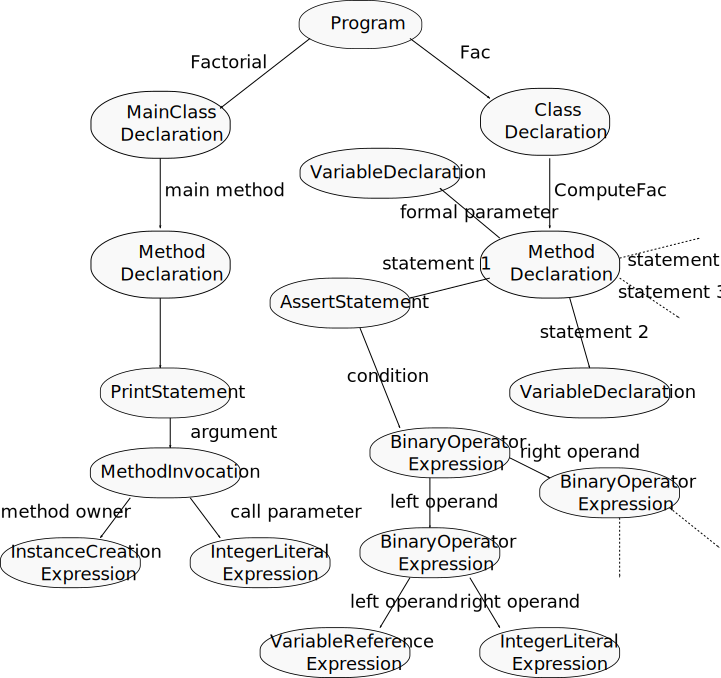
\includegraphics[width=1.0\textwidth]{ast.pdf}

\subsubsection{Interfaces}
\begin{description}
\item[ISyntaxTreeNode] \emph{is a node that can be visited.}
\item[IStatement] \emph{is an} ISyntaxTreeNode \emph{and represents a Mini-Java statement}
\item[IExpression] \emph{is an} ISyntaxTreeNode \emph{and represents a Mini-Java expression}
\end{description}

\subsubsection{Interface implementers}
\begin{description}
\item[Program] \emph{is an} ISyntaxTreeNode \\
\emph{is a root node.} \\
\emph{has a} \textbf{MainClassDeclaration} \\
\emph{has many} \textbf{ClassDeclaration}s
\\
\item[SyntaxElement] \emph{is an abstract} ISyntaxTreeNode \\
\emph{stores row and column information for nodes.}
\\
\item[MainClassDeclaration] \emph{is a} SyntaxElement \\
\emph{has a} \textbf{MethodDeclaration} \emph{which is the main method.} \\
\emph{defines a scope in the semantic analysis phase.}
\item[ClassDeclaration] \emph{is a} SyntaxElement \\
\emph{has many} \textbf{Declaration}s \\
\emph{defines a scope in the semantic analysis phase.}
\\
\item[Declaration] \emph{is an abstract} SyntaxElement \\
\emph{stores type information.}
\item[MethodDeclaration] \emph{is a} Declaration \\
\emph{has many} \textbf{VariableDeclaration}s \emph{which represent formal parameters.} \\
\emph{has many} \textbf{IStatement}s \emph{which form the method body.} \\
\emph{defines a scope in the semantic analysis phase.}
\item[VariableDeclaration] \emph{is a} Declaration \emph{and an} IStatement
\\
\item[AssertStatement] \emph{is a} SyntaxElement \emph{and an} IStatement \\
\emph{has an} \textbf{IExpression} \emph{which is the boolean argument.}
\item[BlockStatement] \emph{is a} SyntaxElement \emph{and an IStatement} \\
\emph{has many} \textbf{IStatement}s \emph{which form the body of the block.} \\
\emph{defines a scope in the semantic analysis phase.}
\item[IfStatement] \emph{is a} SyntaxElement \emph{and an} IStatement \\
\emph{has an} \textbf{IExpression} \emph{which represents the condition.} \\
\emph{has a} \textbf{BlockStatement} \emph{which is the then branch.} \\
\emph{has optionally a} \textbf{BlockStatement} \emph{which is the else branch.}
\item[WhileStatement] \emph{is a} SyntaxElement \emph{and an} IStatement \\
\emph{has an} \textbf{IExpression} \emph{which represents the condition.} \\
\emph{has a} \textbf{BlockStatement} \emph{which is the loop body}
\item[PrintStatement] \emph{is a} SyntaxElement \emph{and an} IStatement \\
\emph{has an} \textbf{IExpression} \emph{which is the integer argument.}
\item[ReturnStatement] \emph{is a} SyntaxElement \emph{and an} IStatement \\
\emph{has an} \textbf{IExpression} \emph{which is the expression to return.}
\item[MethodInvocation] \emph{is a} SyntaxElement \emph{and an} IStatement \emph{and an} IExpression \\
\emph{has an} \textbf{IExpression} \emph{which is the method owner} \\
\emph{has many} \textbf{IExpression}s \emph{which are the call parameters.}
\\
\item[ArrayIndexingExpression] \emph{is a} SyntaxElement \emph{and an} IExpression \\
\emph{has an} \textbf{IExpression} \emph{which is the array reference.} \\
\emph{has an} \textbf{IExpression} \emph{which is the index.}
\item[InstanceCreationExpression] \emph{is a} SyntaxElement \emph{and an} IExpression \\
\emph{has optionally an} \textbf{IExpression} \emph{which is the array size if this is an array creation.} \\
\emph{represents the 'new' expression.}
\item[ThisExpression] \emph{is a} SyntaxElement \emph{and an} IExpression \\
\emph{represents the reference to 'this' class.}
\item[VariableReferenceExpression] \emph{is a} SyntaxElement \emph{and an} IExpression
\item[UnaryOperatorExpression] \emph{is a} SyntaxElement \emph{and an} IExpression \\
\emph{has an} \textbf{IExpression} \emph{which is the operand.}
\item[BinaryOperatorExpression] \emph{is a} SyntaxElement \emph{and an} IExpression \\
\emph{has an} \textbf{IExpression} \emph{that is the left operand.} \\
\emph{has an} \textbf{IExpression} \emph{that is the right operand.}
\item[BooleanLiteralExpression] \emph{is a} SyntaxElement \emph{and an} IExpression
\item[IntegerLiteralExpression] \emph{is a} SyntaxElement \emph{and an} IExpression
\end{description}

\section{Compiler implementation}

This section covers the general architecture of the compiler, testing, error handling as well as the building and running instuctions.

\subsection{Architecture}

The front-end module is divided into three sub-modules, one for each major phase of compilation: lexical analysis, syntax analysis and semantic analysis. In addition, I have collected some things possibly needed by both the front-end and the back-end into the Support module. These include:
\begin{itemize}
\item The abstract syntax tree representation and the related INodeVisitor interface.
\item The symbol table.
\item Static information on the language such as listings of keywords, punctuation characters, operators and operator semantics, precedences etc. This can be expanded to include possible semantic information needed by the back-end later.
\item Error handling: an error reporter interface and a basic implementation for it.
\end{itemize}

\subsubsection{Simplified view of the front-end module}

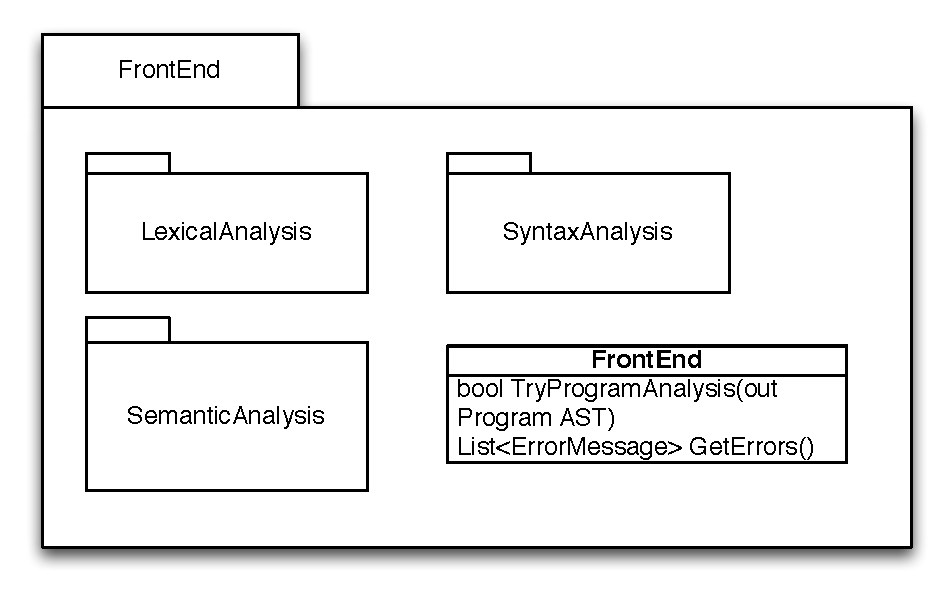
\includegraphics[width=1.0\textwidth]{frontend.pdf}

\subsubsection{Simplified view of the support module}

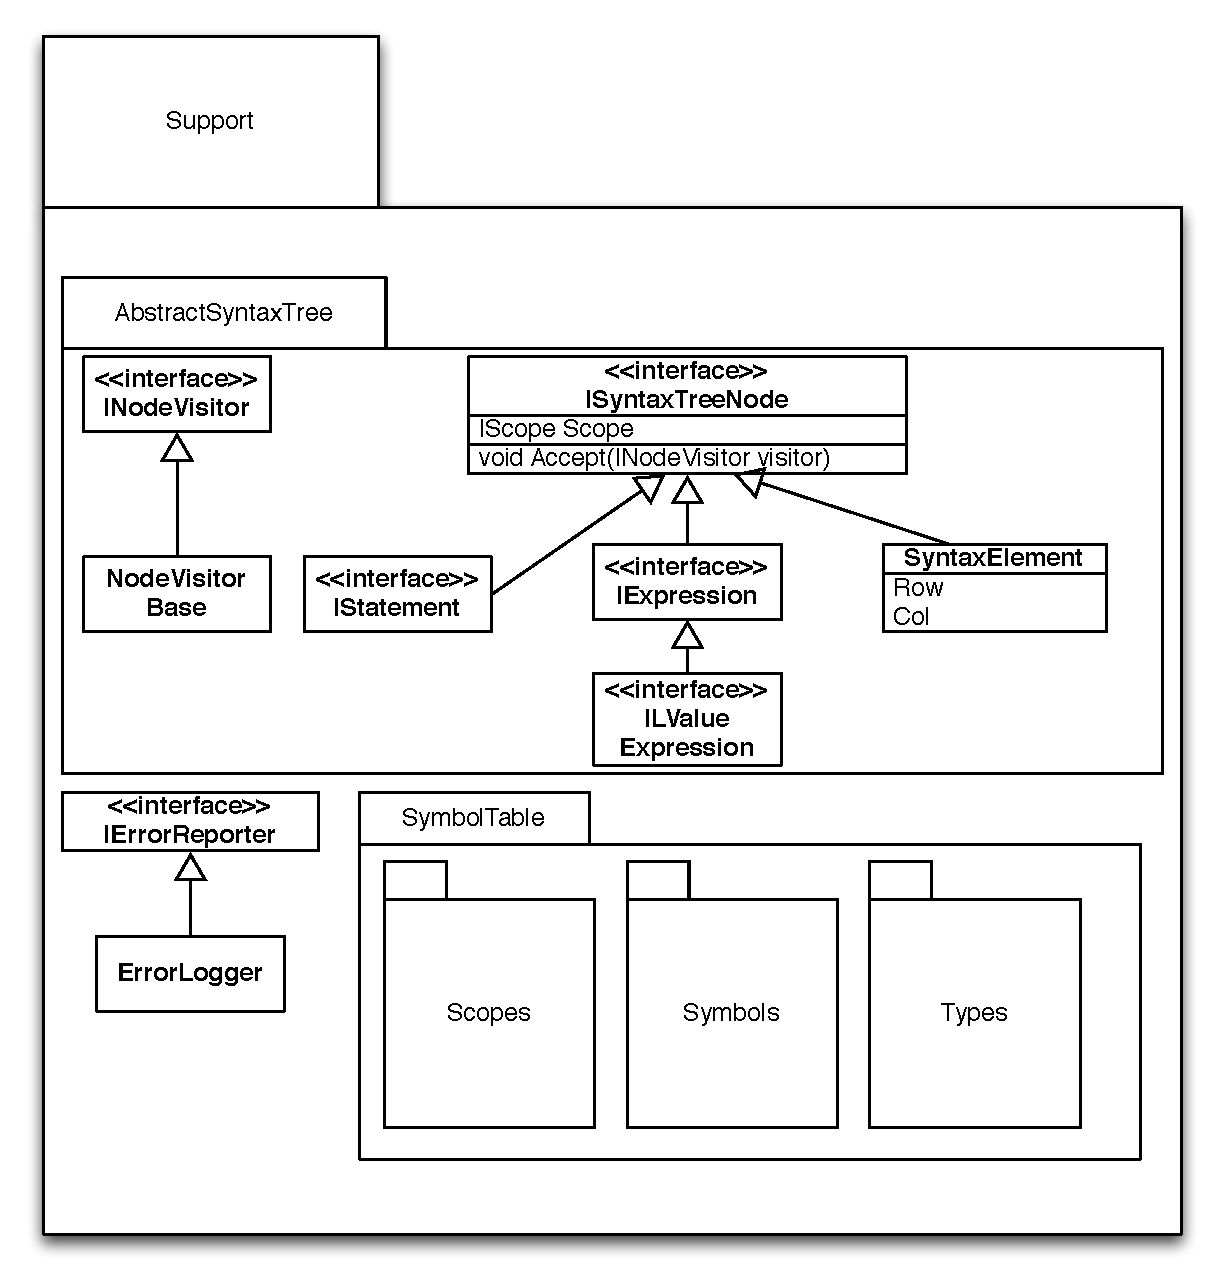
\includegraphics[width=1.0\textwidth]{support.pdf}

\subsection{Lexical analysis}

% error handling in this phase

\subsection{Syntax analysis}

% error handling in this phase

\subsection{Semantic analysis}

% error handling in this phase

\subsection{Testing}

\subsection{Building and running the compiler}

\subsection{Possible bugs}

\end{document}
